\chapter{Related Work}
\label{ch:state_of_the_art}
%
The ocean surface is an intricate phenomenon which owes its complexity
to its highly dynamic nature. Be it a quiet sea or an agitated one, small
turbulent waves or huge breaking ones, the underlying mechanisms are manifold
and act on a variety of scales. Oceanographic research defines the behaviour of
an ocean surface based on its location. Water areas far from the coast are
called~\emph{the deep ocean}, water areas close to shore are called
\emph{shallow water}. Deep ocean surfaces are governed by the interaction of
wind and gravity at the interface between air and water, whereas shallow water
surfaces are characterized by waves breaking near the shore. FIXME: give an
overview of what is to come.
%
\section{Simulation}
%
To date, computer graphics employs several ocean wave models which may be
separated roughly into three families: parametric description, spectral
description, computational fluid dynamics. The first describes the water surface
by means of parametric equations which have been derived based on real world
observations \citep{Gerstner:1809,Rankine:1863,Biesel:1952}.
The second family approximate the ocean surface using wave spectra which
simulate the sea as a random process based on the distribution of wave energy
in frequency space \citep{book:kinsman2002wind,article:PiersonMoskowitz1964,
article:Hasselman1973,article:Donelan1985,article:Elfouhaily1997}.
Third, computational fluid dynamics and more specifically the Navier-Stokes
equations are able to fully describe the dynamics of all kinds of fluid,
including the ocean. FIXME: Short discussion of NSE and dismiss them, because
out of scope.
%
\subsection{Parametric Models}
%
\begin{figure}
\centering
 \subtop[]
 {
  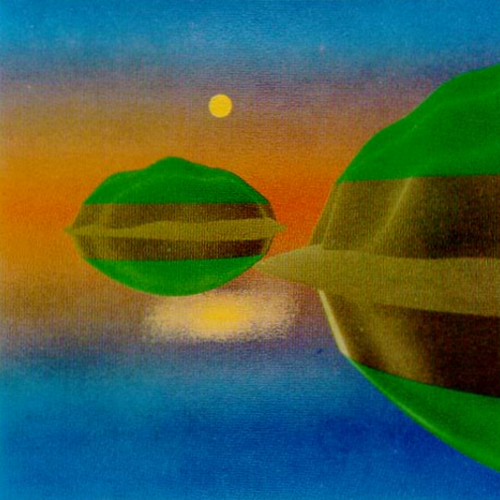
\includegraphics[scale=0.25]{figures/Vectorized_Procedural_Models_for_Natural_Terrain_-_Max_1981-006_1.png}
	\label{fig:max1981:1}
 }
 \hfill
 \subtop[]
 {
  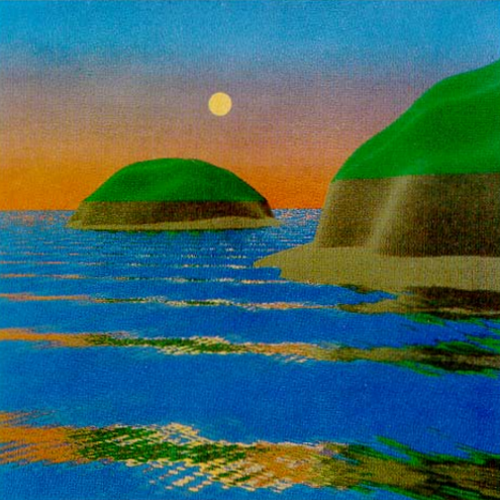
\includegraphics[scale=0.25]{figures/Vectorized_Procedural_Models_for_Natural_Terrain_-_Max_1981-007_1.png}
	\label{fig:max1981:2}
 }
 \hfill
 \subtop[]
 {
  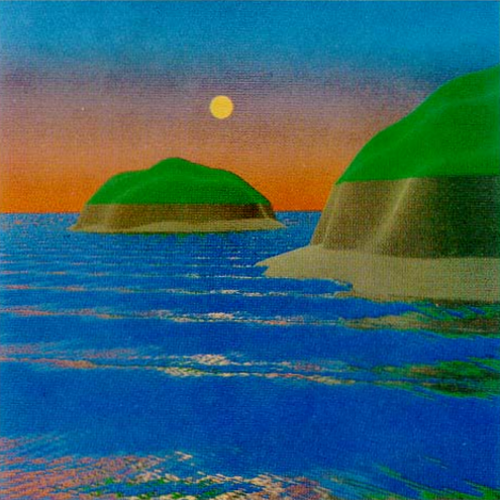
\includegraphics[scale=0.25]{figures/Vectorized_Procedural_Models_for_Natural_Terrain_-_Max_1981-006_2.png}
	\label{fig:max1981:3}
 }
 \hfill
 \subtop[]
 {
  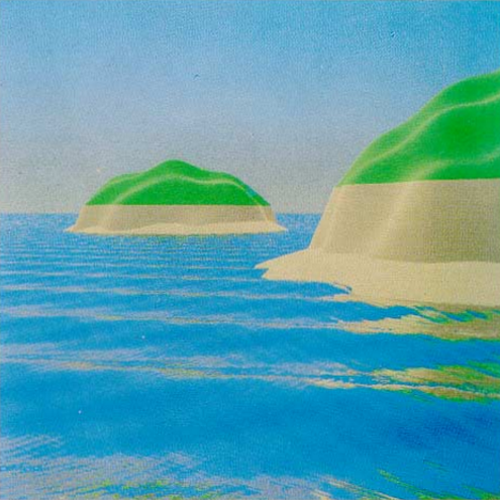
\includegraphics[scale=0.25]{figures/Vectorized_Procedural_Models_for_Natural_Terrain_-_Max_1981-007_2.png}
	\label{fig:max1981:4}
 }
\caption{\subcaptionref{fig:max1981:1}~Still water near sunset.
\subcaptionref{fig:max1981:2} One reflection from waves.
\subcaptionref{fig:max1981:3} Two reflections from waves.
\subcaptionref{fig:max1981:4} Early afternoon, two reflections from waves.
Source:~\cite{Max:1981}}
\label{fig:max1981}
\end{figure}
%
The parametric models are generally bound to the spatial domain, where they
generate and animate the ocean surface by means of a sum of periodical functions
which evolve throughout time using a phase difference. One of the earliest works
in this realm of computer graphics has been done by~\citet{Max:1981}. The ocean
surface is represented as a height map, where for each point $(x,z)$ at time $t$
the height is computed as a sum of sinusoids:
\begin{equation}
h(x,z,t) = y + \sum_{i=1}^N A_i \cos (l_i x + m_i z - \omega_i t)
\end{equation}
where $y$ is the mean height of the free surface, $N$ is the number of waves,
$A_i$ is the amplitude of the $i$th wave, $\mvec{k}_i = (l_i, m_i)$ its wave
vector, and $\omega_i$ its angular frequency. The wave vector defines the
travelling direction of the wave, with the the positive X-axis pointing towards
the coastline, the Y-axis pointing in the opposite direction of earth's gravity,
and the Z-axis aligned with the coastline. For the sum of waves to achieve a
realistic shape, \citeauthor{Max:1981} applies linear wave theory.
The waves on the water surface are assumed to be dominated by gravity, the wave
amplitudes are assumed to be small in relation to the size of the water body,
and the water body is assumed to have infinite depth. Then, according to linear
wave theory it follows that the wave number $k=\norm{\mvec{k}}$ and the angular
frequency $\omega$ are related by $\omega^2=kg$, where $g=9.81$ denotes earth's
gravity. Results obtained by~\citeauthor{Max:1981} are shown in
Figure~\ref{fig:max1981}.
%
\begin{figure}
 \centering
 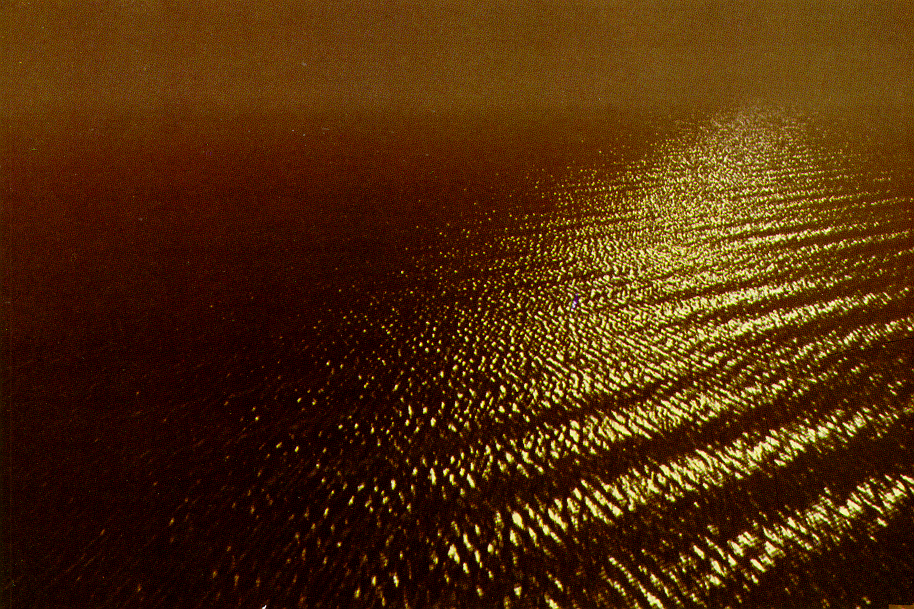
\includegraphics[scale=0.25]{figures/An_Image_Synthesizer_-_Perlin_1985-021.png}
 \caption{Ocean sunset. Source:~\cite{Perlin:1985}}
\label{fig:perlin1985}
\end{figure}
%

Both,~\cite{Schachter:1980} and~\cite{Perlin:1985}, developed similar approaches,
where instead of generating any actual geometry they simply distort the normal
vectors of given surfaces. Results obtained by~\citeauthor{Perlin:1985} are
shown in Figure \ref{fig:perlin1985}.
%
\begin{figure}
 \centering
 \subtop[]
 {
  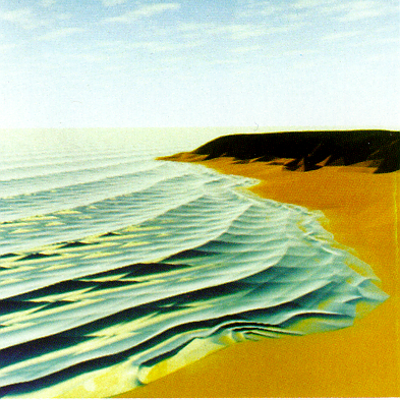
\includegraphics[scale=0.25]{figures/Modeling_Waves_and_Surf_-_Peachey_1986-009.png}
	\label{fig:peachey1986:1}
 }
 \hfill
 \subtop[]
 {
  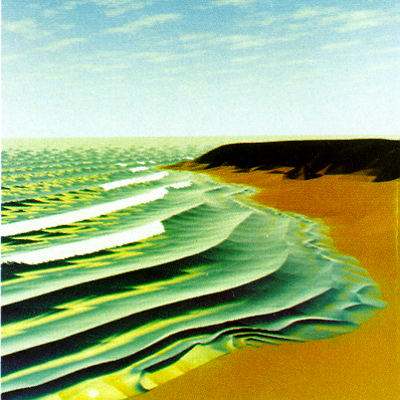
\includegraphics[scale=0.25]{figures/Modeling_Waves_and_Surf_-_Peachey_1986-010.png}
	\label{fig:peachey1986:2}
 }
 \hfill
 \subtop[]
 {
  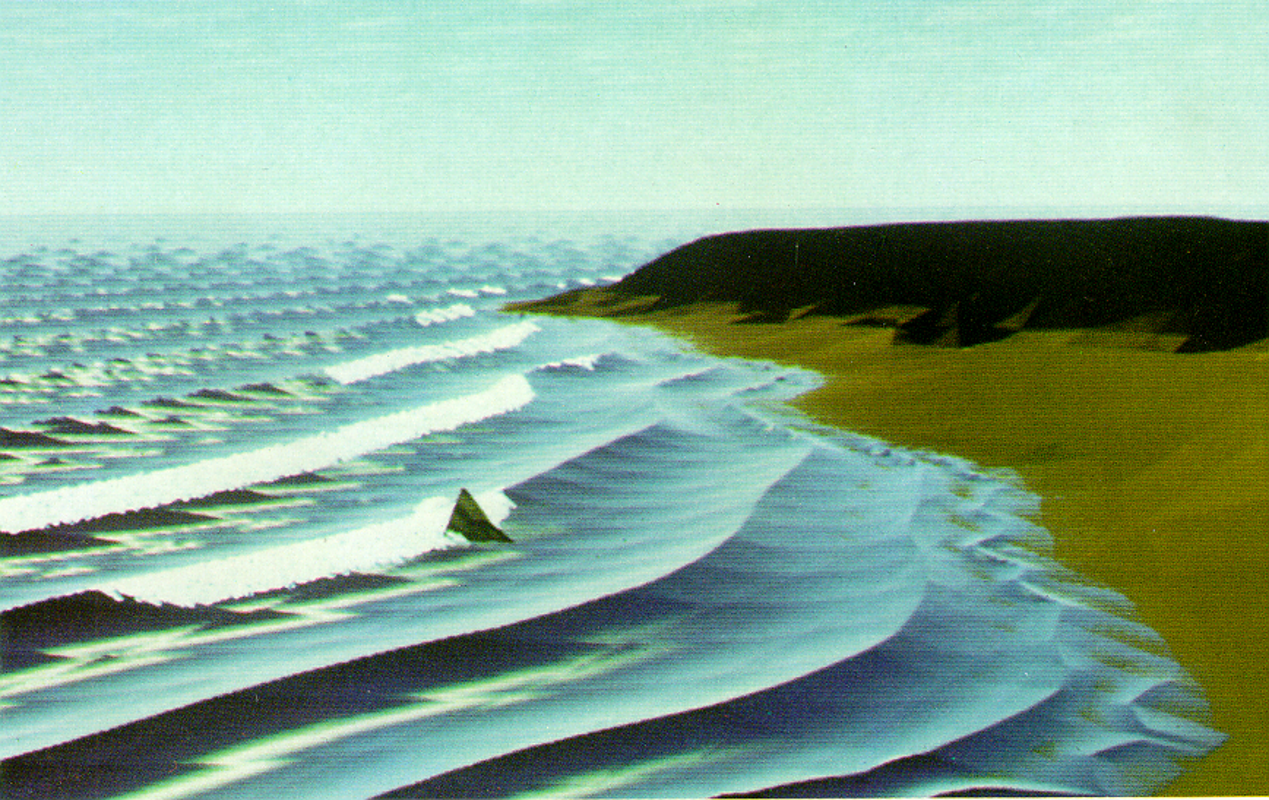
\includegraphics[scale=0.125]{figures/Modeling_Waves_and_Surf_-_Peachey_1986-012.png}
	\label{fig:peachey1986:3}
 }
 \caption{\subcaptionref{fig:peachey1986:1}~Waves on the beach.
\subcaptionref{fig:peachey1986:2}~Breaking waves on the beach.
\subcaptionref{fig:peachey1986:3}~Breaking waves with obstacle.
Source:~\cite{Peachey:1986}}
\label{fig:peachey1986}
\end{figure}
%
The assumption of infinite depth restricts the above methods to deep water, they
are unable to include phenomena which arise near the shore, such as breaking
waves and wave refraction. \cite{Peachey:1986}, still in the realm of linear
wave theory, simulates waves near the shore through the relationship
$\omega^2=kg\tanh (kh)$, where $h$ is the water depth. Moreover,
\citeauthor{Peachey:1986} distorts waves approaching the sloping beach so that
they resemble breaking waves more closely. Additionally, particle systems are
added to generate spray. Results of \cite{Peachey:1986} are shown in
Figure~\ref{fig:peachey1986}.
%
\begin{figure}
 \centering
 \subtop[]
 {
  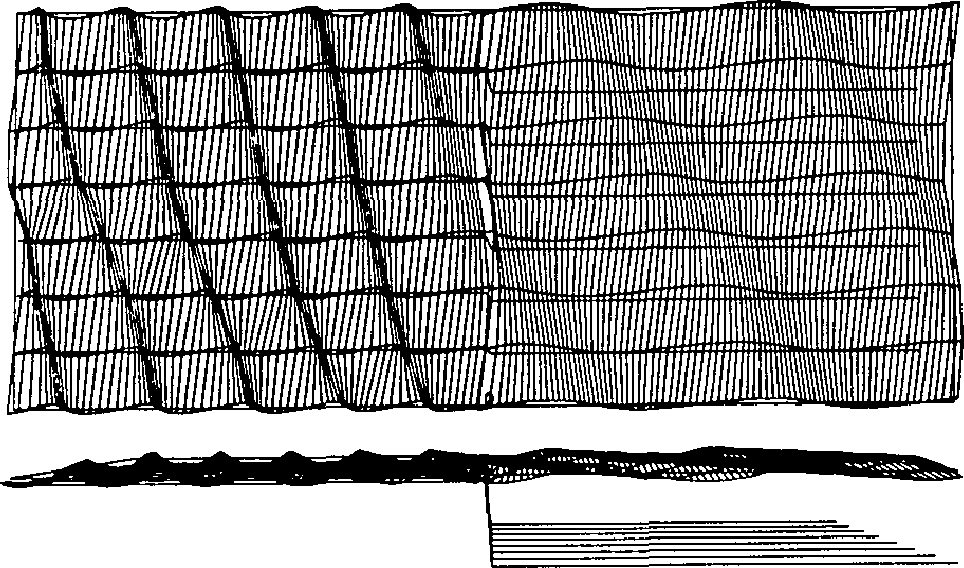
\includegraphics[scale=0.175]{figures/A_Simple_Model_of_Ocean_Waves_-_Fournier_1986-004_1.png}
	\label{fig:fournier1986:refraction:1}
 }
 \hfill
 \subtop[]
 {
  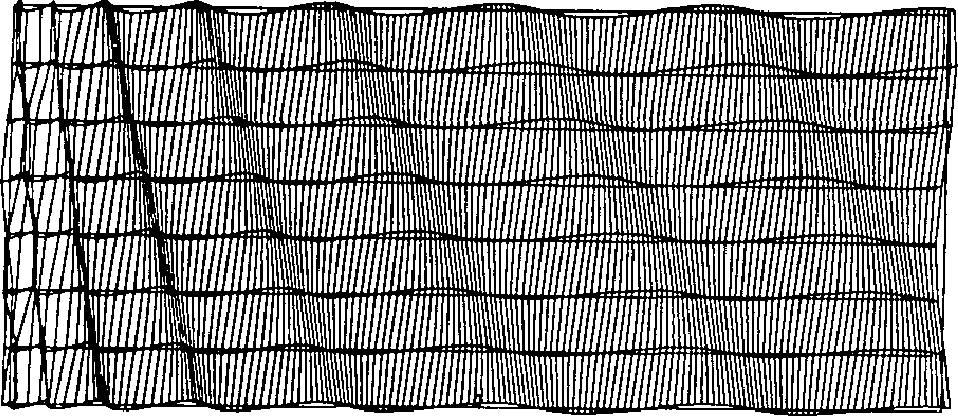
\includegraphics[scale=0.175]{figures/A_Simple_Model_of_Ocean_Waves_-_Fournier_1986-004_2.png}
	\label{fig:fournier1986:refraction:2}
 }
 \hfill
 \subtop[]
 {
  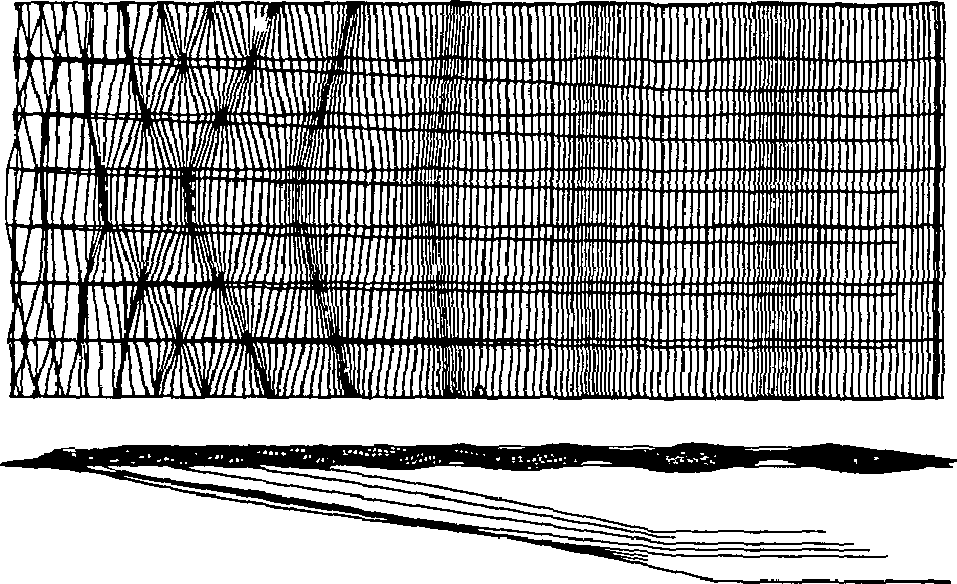
\includegraphics[scale=0.175]{figures/A_Simple_Model_of_Ocean_Waves_-_Fournier_1986-005_1.png}
	\label{fig:fournier1986:refraction:3}
 }
 \caption{The refraction of waves.
\subcaptionref{fig:fournier1986:refraction:1} Two bottoms of constant depth, the
wavelengths are halved as the waves reach the shallow bottom on the left.
\subcaptionref{fig:fournier1986:refraction:2} The beach slopes gently down from
the left. One can see the wave fronts aligning themselves with the beach.
\subcaptionref{fig:fournier1986:refraction:3} An undersea valley that affects
both, the wavelengths as well as the travelling direction of the waves.
Source:~\cite{Fournier:1986}}
\label{fig:fournier1986:refraction}
\end{figure}
%

\cite{Fournier:1986}, instead of using sinusoids, build on Gerstner's work
\citep{Gerstner:1809, Rankine:1863} to synthesize waves. Gerstner waves assume
a water surface dominated by gravity and an incompressible water body of
infinite depth. A single wave may be written as follows:
\begin{align}
\mvec{x} &= \mvec{x}_0 - \frac{\mvec{k}}{\norm{\mvec{k}}} A \sin\left(\mvec{k}\cdot\mvec{x}_0-\omega t\right)\\
y &= y_0 - A \cos\left(\mvec{k}\cdot\mvec{x}_0-\omega t\right)
\end{align}
where $\mvec{x}$ denotes the horizontal coordinate and $y$ the vertical coordinate
of the wave particle at time $t$, with $\mvec{x}_0$ and $y_0$ its horizontal
and vertical position at rest respectively. As before, $A$ is the amplitude,
$\mvec{k}$ the wave vector and $\omega$ the wave's angular frequency. Given the
wave number $k=\norm{\mvec{k}}$, the term $kA$ defines the sharpness of the wave
crest. With $kA<1$ the wave takes the form of an upside-down trochoid, with
$kA=1$ the form of an upside-down cycloid, and with $kA>1$ the wave intersects
itself, an undesired effect which does not resemble real waves.
See Figure~\ref{fig:trochoid:crests} for waves with different $kA$.
%Gerstner waves take the form of an upside-down trochoid.
%
\begin{figure}
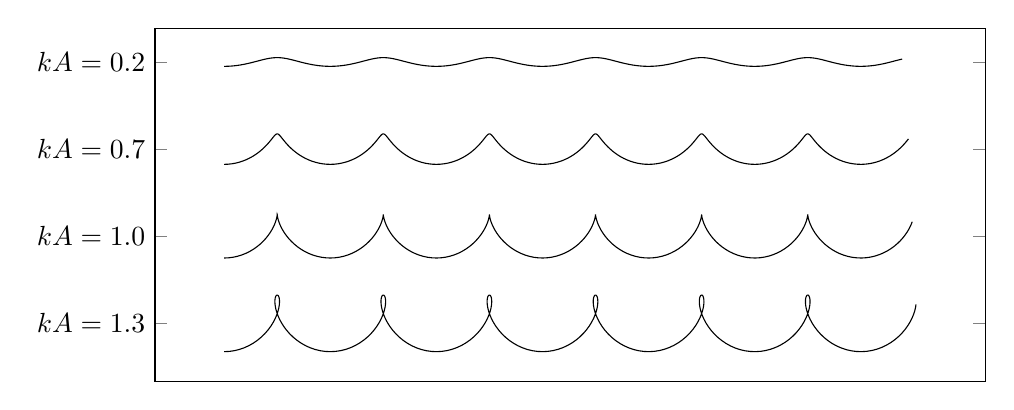
\begin{tikzpicture}
\begin{axis}[
	width=\textwidth,
	height=0.5\textwidth,
	domain=0:40,
	%xmin = 0,
	%xmax = 40,
	%axis equal,
	xtick=\empty,
	%ytick=\empty,
	%y tick label style={anchor=west,xshift=\pgfkeysvalueof{/pgfplots/major tick length}},
	yticklabels={$kA=0.2$,$kA=0.7$,$kA=1.0$,$kA=1.3$},
	ytick={12,8,4,0} 
	]
\addplot[samples=300,domain=0:40] ({x+0.2*sin(deg(1*x-sqrt(9.81*1)*0))}, {12-0.2*cos(deg(1*x-sqrt(9.81*1)*0))});
\addplot[samples=300,domain=0:40] ({x+0.7*sin(deg(1*x-sqrt(9.81*1)*0))}, { 8-0.7*cos(deg(1*x-sqrt(9.81*1)*0))});
\addplot[samples=300,domain=0:40] ({x+1.0*sin(deg(1*x-sqrt(9.81*1)*0))}, { 4-1.0*cos(deg(1*x-sqrt(9.81*1)*0))});
\addplot[samples=300,domain=0:40] ({x+1.3*sin(deg(1*x-sqrt(9.81*1)*0))}, { 0-1.3*cos(deg(1*x-sqrt(9.81*1)*0))});
\end{axis}
\end{tikzpicture}
\caption{Brak.}
\label{fig:trochoid:crests}
\end{figure}
%

The sum of of Gerstner waves is as follows:
\begin{align}
\mvec{x} &= \mvec{x}_0 - \sum_i^N\frac{\mvec{k}_i}{\norm{\mvec{k_i}}} A_i \sin\left(\mvec{k}_i\cdot\mvec{x}_0-\omega t\right)\\
y &= y_0 - \sum_i^N A_i \cos\left(\mvec{k}_i\cdot\mvec{x}_0-\omega t\right)
\end{align}
%
\begin{figure}
 \centering
 \subtop[]
 {
  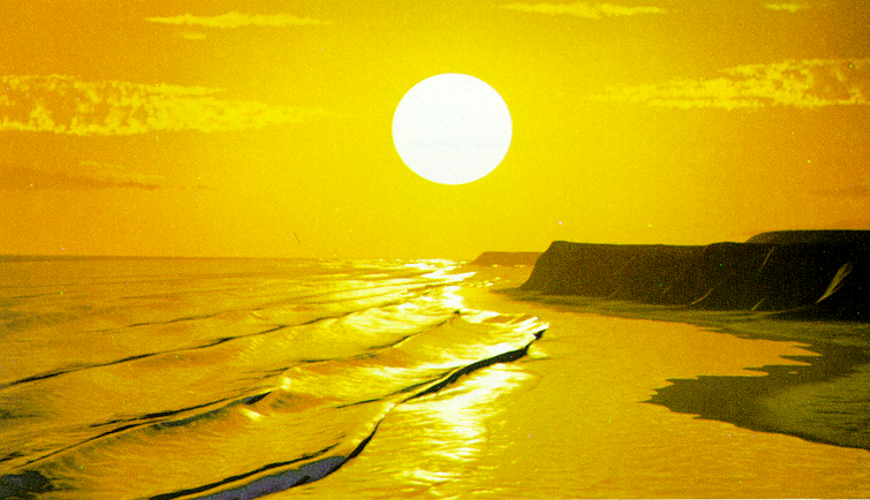
\includegraphics[scale=0.225]{figures/A_Simple_Model_of_Ocean_Waves_-_Fournier_1986-008.png}
	\label{fig:fournier1986:results:1}
 }
 \hfill
 \subtop[]
 {
  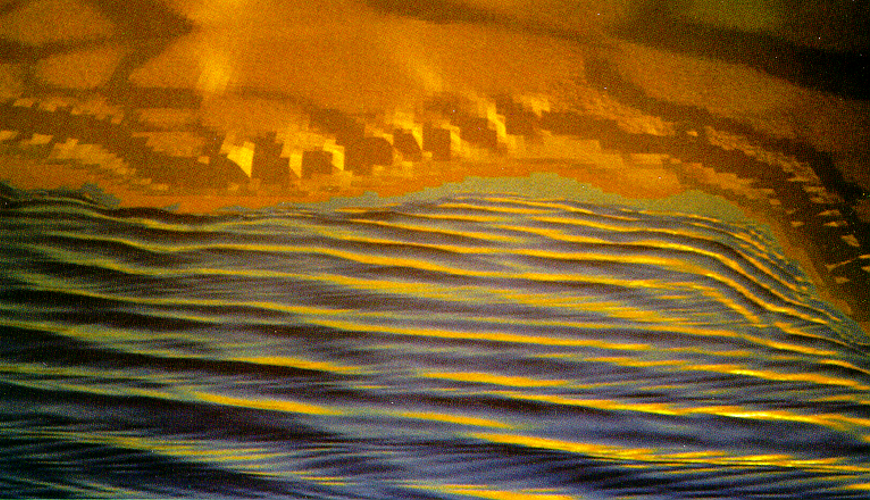
\includegraphics[scale=0.225]{figures/A_Simple_Model_of_Ocean_Waves_-_Fournier_1986-010.png}
	\label{fig:fournier1986:results:2}
 }
 \subtop[]
 {
  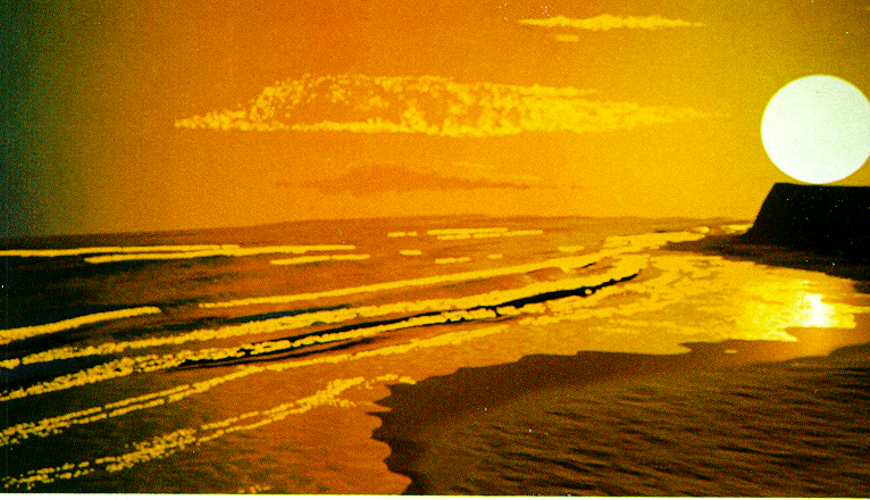
\includegraphics[scale=0.225]{figures/A_Simple_Model_of_Ocean_Waves_-_Fournier_1986-011.png}
	\label{fig:fournier1986:results:3}
 }
 \hfill
 \subtop[]
 {
  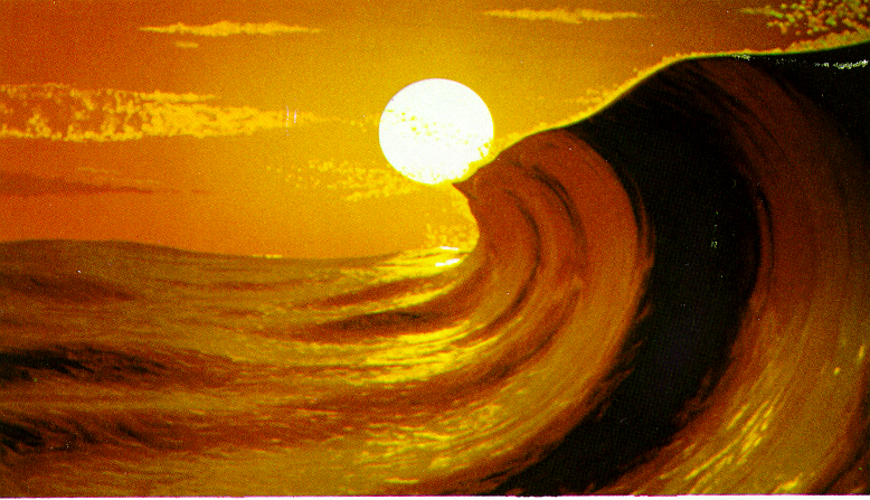
\includegraphics[scale=0.225]{figures/A_Simple_Model_of_Ocean_Waves_-_Fournier_1986-013.png}
	\label{fig:fournier1986:results:4}
 }
 \caption{
 \subcaptionref{fig:fournier1986:results:1} Breaking waves on the shore, where the crests take the shape of the shore.
 \subcaptionref{fig:fournier1986:results:2} Wave refraction.
 \subcaptionref{fig:fournier1986:results:3} Waves with spray and foam.
 \subcaptionref{fig:fournier1986:results:4} A large breaking wave.
 Source:~\cite{Fournier:1986}
 }
 \label{fig:fournier1986:results}
\end{figure}
%
\citeauthor{Fournier:1986} improve upon the above model in two ways. First, wave
particle motion takes the underlying sea bed into account, allowing for waves
to be refracted i.e. to change their wavelength, their speed and their direction
of travel, see Figure~\ref{fig:fournier1986:refraction}. Second, the circular
orbit of Gerstner waves approaching the shore is transformed into an elliptical
orbit, which allows the formation of breaking waves near the beach. Results of
\cite{Fournier:1986} are shown in Figure~\ref{fig:fournier1986:results}.

\cite{Ts'o:1987} implement an algorithm called \emph{wave tracing} which
launches orthogonal wave rays from the open sea along the direction of wave
propagation. Wave refraction is computed based on Snell's law, the wave trains
are traced inside a uniform grid. In case rays tracing the waves path diverge
significantly from a straight line, there may remain undersampled areas,
leading to parts of the surface lacking detail. \cite{Gonzato:1997} improve
upon this by generating new rays in undersampled areas, allowing the algorithm
to more densely sample the water surface surrounding an island and the water
surface inside bays. Moreover, \citeauthor{Gonzato:1997} modify the wave model to
include plunging breaking waves. Three additional functions achieve said goal.
A stretch function which imitates Biesel law~\citep{Biesel:1952} by
progressively stretching the wave on the crest along its major axis. An
orientation and a displacement function to rotate the wave's crest downwards,
towards the water surface below the crest.

Spectral Models
Navier Stokes

Rendering

Particles
Reflection
Refraction
Foam, Sprays

Parametric\\
%Perlin - An Image Synthesizer \cite{Perlin:1985}\\
%Nelson Max - Vectorized Procedural Models for Natural Terrain: Waves and Islands in the Sunset \cite{Max:1981}\\
%Peachey - Modeling Waves and Surf \cite{Peachey:1986}\\
%Fournier - A simple model of ocean waves \cite{Fournier:1986}\\
%Ts'o - Modeling and rendering waves: Wave-tracing using beta-splines and reflective and refractive texture mapping \cite{Ts'o:1987}
Hinsinger - Interactive Animation of Ocean Waves \cite{Hinsinger:2002}\\

Spectral\\
Mastin - Fourier Synthesis of Ocean Scenes \cite{Mastin:1987}\\
Tessendorf - Simulating Ocean Water \cite{course:simulatingocean}\\
Premoze - Rendering Natural Waters \cite{Premoze:2000} \\

Hybrid\\
Thon - Ocean waves synthesis using a spectrum based turbulence function \cite{thon:2000}\\
Lee - Real-Time Simulation of Surface Gravity Ocean Waves Based on the TMA Spectrum\cite{lee:2007}\\



%\begin{figure}
%\centering
 %\subtop
 %{
  %\includegraphics[scale=0.45]{figures/ocean300_5.jpg}
 %}
 %\hfill
 %\subtop
 %{
  %\includegraphics[scale=0.45]{figures/ocean_storm300.jpg}
 %}
%\caption{The late afternoon sun illuminating the ocean surface. Source:~\cite{misc:noaa}}
%\end{figure}







\begin{figure}
 \centering
 \subtop
 {
  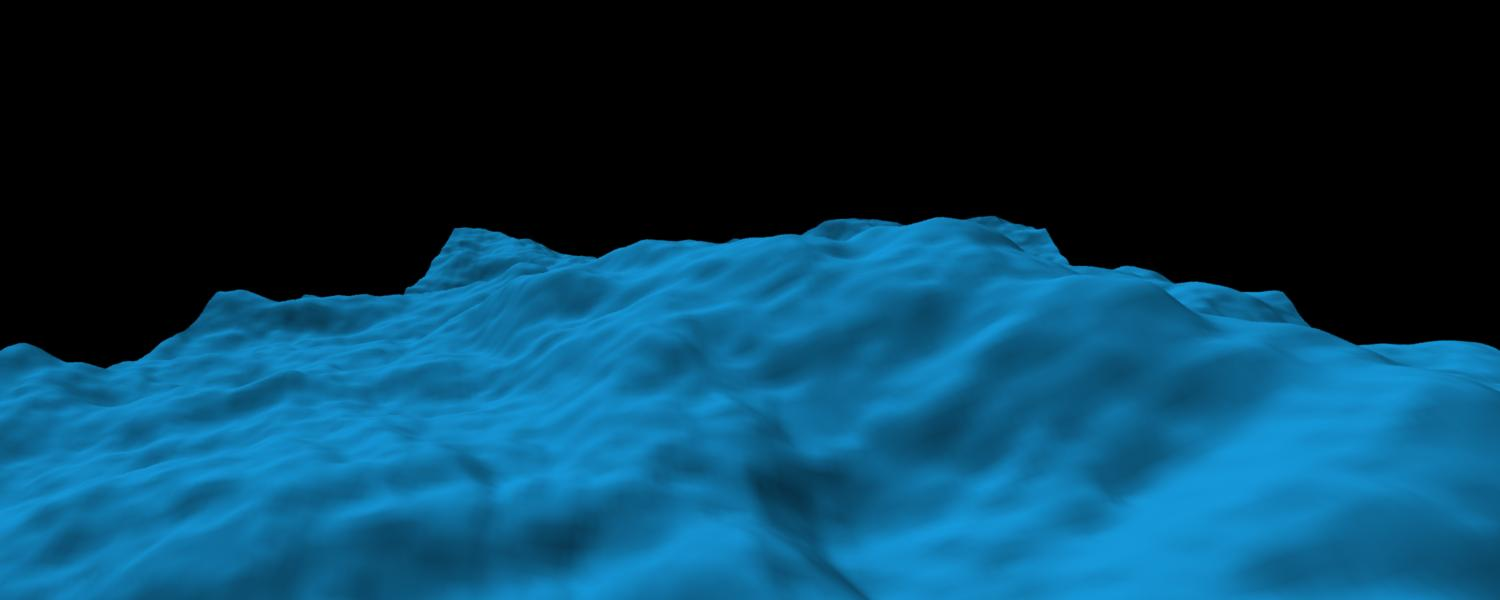
\includegraphics[scale=0.125]{figures/Simulating_Ocean_Water-012.png}
 }
 \subtop
 {
  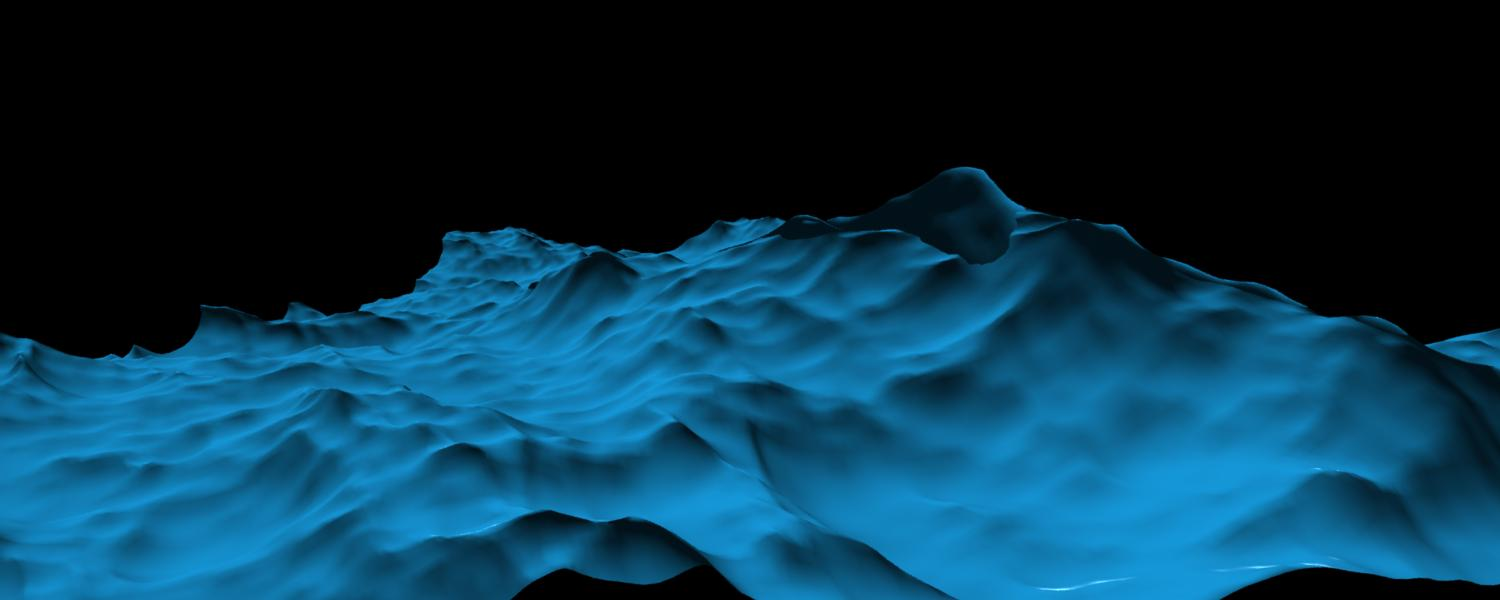
\includegraphics[scale=0.125]{figures/Simulating_Ocean_Water-013.png}
 }
 \caption{Tessendorf 1999}
\end{figure}

\begin{figure}
 \centering
 \subtop
 {
  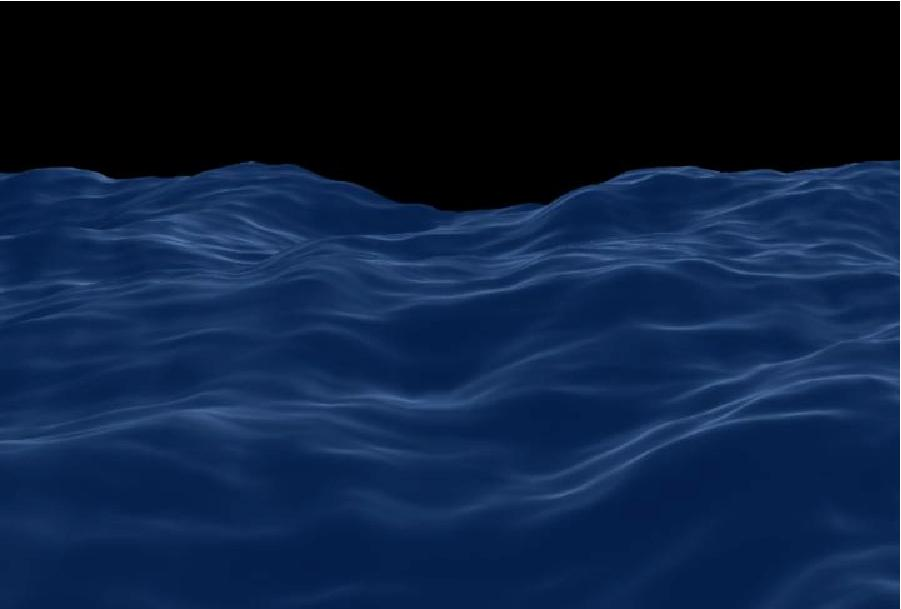
\includegraphics[scale=0.145]{figures/Simulating_Ocean_Water-008.png}
 }
 \hfill
 \subtop
 {
  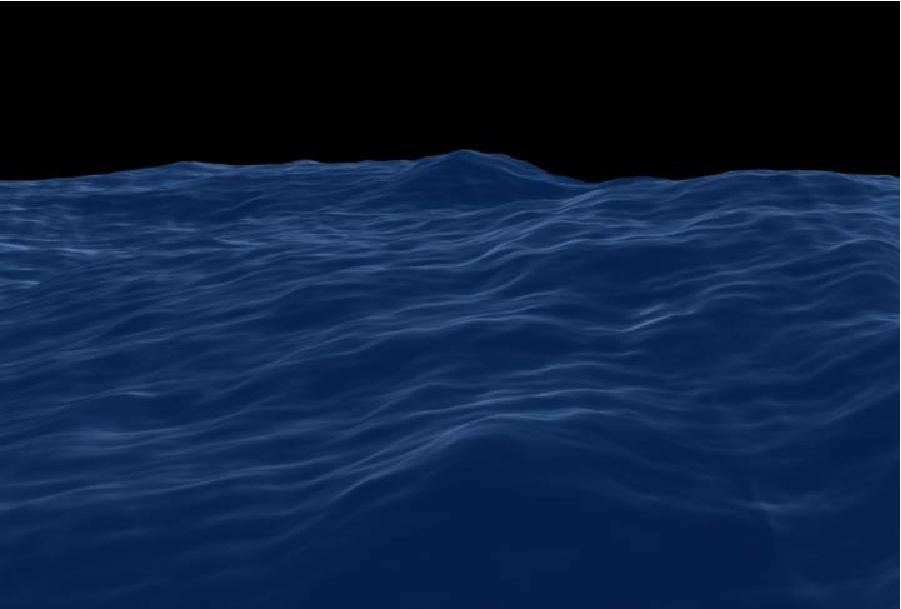
\includegraphics[scale=0.145]{figures/Simulating_Ocean_Water-009.png}
 }
 \hfill
 \subtop
 {
  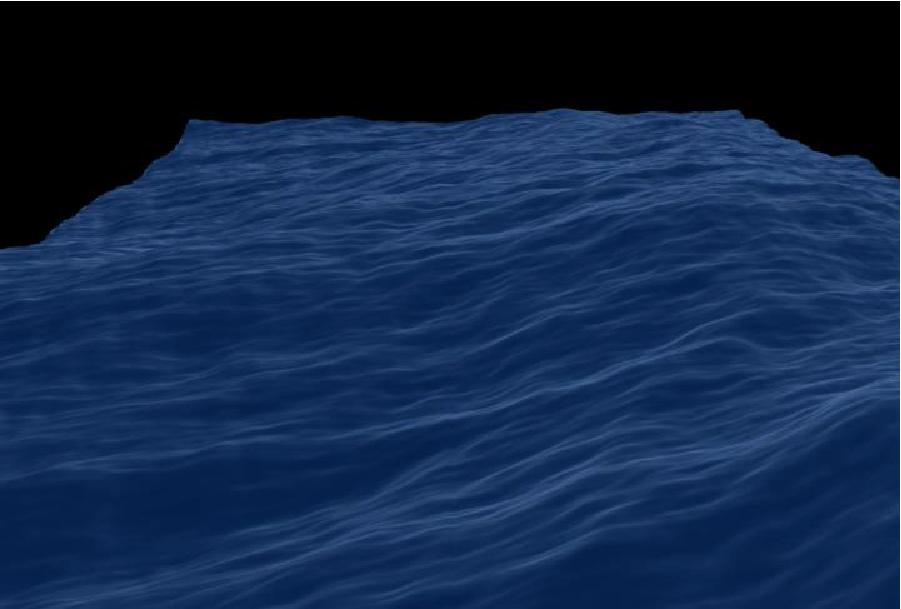
\includegraphics[scale=0.145]{figures/Simulating_Ocean_Water-010.png}
 }
 \caption{Tessendorf 1999}
\end{figure}